%%%%%%%%%%%%%%%%%%%%%%% file template.tex %%%%%%%%%%%%%%%%%%%%%%%%%
%
% This is a general template file for the LaTeX package SVJour3
% for Springer journals.          Springer Heidelberg 2010/09/16
%
% Copy it to a new file with a new name and use it as the basis
% for your article. Delete % signs as needed.
%
% This template includes a few options for different layouts and
% content for various journals. Please consult a previous issue of
% your journal as needed.
%
%%%%%%%%%%%%%%%%%%%%%%%%%%%%%%%%%%%%%%%%%%%%%%%%%%%%%%%%%%%%%%%%%%%
%
% First comes an example EPS file -- just ignore it and
% proceed on the \documentclass line
% your LaTeX will extract the file if required
\begin{filecontents*}{example.eps}
%!PS-Adobe-3.0 EPSF-3.0
%%BoundingBox: 19 19 221 221
%%CreationDate: Mon Sep 29 1997
%%Creator: programmed by hand (JK)
%%EndComments
gsave
newpath
  20 20 moveto
  20 220 lineto
  220 220 lineto
  220 20 lineto
closepath
2 setlinewidth
gsave
  .4 setgray fill
grestore
stroke
grestore
\end{filecontents*}
%
\RequirePackage{fix-cm}
%
%\documentclass{svjour3}                     % onecolumn (standard format)
%\documentclass[smallcondensed]{svjour3}     % onecolumn (ditto)
\documentclass[smallextended]{svjour3}       % onecolumn (second format)
%\documentclass[twocolumn]{svjour3}          % twocolumn
%
\smartqed  % flush right qed marks, e.g. at end of proof
%
\usepackage{graphicx}
\usepackage{natbib}

%
% \usepackage{mathptmx}      % use Times fonts if available on your TeX system
%
% insert here the call for the packages your document requires
%\usepackage{latexsym}
% etc.
%
% please place your own definitions here and don't use \def but
% \newcommand{}{}
%
% Insert the name of "your journal" with
% \journalname{myjournal}
%
\begin{document}

\title{Childcare Dynamics and Women's Residential Autonomy%\thanks{Grants or other notes
%about the article that should go on the front page should be
%placed here. General acknowledgments should be placed at the end of the article.}
}
%\titlerunning{Short form of title}        % if too long for running head

\author{Layne Vashro
}

%\authorrunning{Short form of author list} % if too long for running head

\institute{L. Vashro \at
              270 S. 1400 E. Rm 102 Department of Anthropology \\
              Tel.: 801-581-6251\\
              \email{layne.vashro@anthro.utah.edu}           %  \\
}

\date{Received: date / Accepted: date}
% The correct dates will be entered by the editor


\maketitle

\begin{abstract}

\emph{Purpose:}  This paper investigates the common hunter-gatherer residence pattern of women delaying natal dispersal until after they have weaned at least one child.  I demonstrate how this pattern is consistent with the expected shift in allocare sources due to changing kin-group demographics over time.  Maternal grandmothers offer a uniquely incentivized source of care to young mothers, but mothers with older daughters can turn to these babysitters as a comparable alternative.  This has important implications for residence, because while a woman's mother is often tied to the natal camp, her older daughters provide a mobile source of care which frees her to respond to other residence incentives.   

\emph{Methods:} I use a computer simulation to model child-caring decisions and highlight the shift in allocare source within a cooperative female kin group across a single generation.

\emph{Results:}  The simulation shows that as a woman progresses through her reproductive career, the source of childcare assistance shifts from those tied to the natal camp to those intrinsic to her and her children.  The simulation also demonstrates the variable nature of allocare as a residence incentive, which has interesting implications for the remarkable flexibility of human residence patterns.

\emph{Conclusions:}  Childcare assistance is likely an important factor in women's residence decisions, particularly in subsistence societies.  However, the natal camp's unique advantage in access to childcare assistance diminishes over time.  This finding is important to understanding patterns of post-marital residence. 

\keywords{Residence \and Allocare \and Dispersal \and Life History}

\end{abstract}

\section{Introduction}
\label{intro}
Females among humans' closest primate relatives disperse from their natal group after reaching reproductive maturity \cite{nishida1987chimpanzees, gerloff1999intracommunity, stokes2003female}.  This is also the case in many human societies \cite{murdock1967ethnographic}, but is far from a universal pattern and only describes a minority of documented foragers \cite{alvarez2004residence, marlowe2004marital}.  Instead, the modal pattern of post-marital residence among human foragers is “multilocal,” where both sexes may or may not disperse from their natal camp \cite{hill2011co}.  These flexible systems are complex and situation specific, but often women remain in their family's household initially then later move away, possibly into the familial household of their husbands \cite{marlowe2004marital}.  This general pattern is supported by informants in a wide variety of forager societies \cite{lee1974male, hewlett1993intimate, marlowe2004marital, hill1996ache}, but has only been assessed with quantitative data in a minority of cases (see \cite{hill2011co_sup} for the Ach\'{e} and Ju/’hoansi and \cite{jones2005hadza} for the Hadza).  Marlowe finds that twenty-five percent of the forager groups in the Standard Cross Cultural Sample fit this pattern \cite{marlowe2004marital, murdock1969standard}, however the real prevalence may be even higher since the ethnographic data rarely gives the level of detail needed to identify age-based trends in “multilocal” residence.  In this paper, I use a computer simulation to demonstrate how this pattern could follow from the dynamics of childcare assistance within the natal camp over time. 

Due to short inter-birth intervals and long periods of childhood dependence, human mothers often find themselves simultaneously caring for multiple young children \cite{key2000evolution}.  In order to meet this challenge, dependence on non-maternal sources of care is an important feature of human life-history \cite{hawkes1998grandmothering, kaplan2000theory}.  Children require food, physical contact, transportation, washing, and constant attention to ensure their safety.  These needs are particularly acute in the first several years of life when mortality risk is at its peak \cite{hill1996ache}.  Fathers often add support in the form or food provisioning and in some cases holding infants \cite{marlowe2003critical, crittenden2008allomaternal}, but are much less involved in other aspects of childcare.  This may be due to the sexual division of labor which separates men from their children throughout much of the day \cite{hewlett1992father}.  This lack of direct childcare could explain why the loss of a father has little or no effect on child survival across many different societies \cite{sear2008keeps}.  Especially when food is widely shared throughout camp, the particular nature of paternal provisioning may be easily substituted by alternative sources when necessary \cite{sugiyama2005juvenile, kaplan1984food, hawkes2001hadza}.  Rather than fathers, it is often mothers' female relatives who have the strongest impact on children's well-being \cite{sear2008keeps}.  A woman's mother and sisters help by directly caring for her children and cooperatively managing the balance between watching over children and accomplishing daily tasks \cite{valeggia2009changing, henry2005child, crittenden2008allomaternal, hawkes1997hadza}.  Since these sources of care are available to women living in their familial camp, but not to those who move to live with their husbands' family, childcare assistance may be one important incentive for women to stay home.  

However, as early-born children age, those children also begin to play an important role in childcare assistance.  Even children as young as three years old begin offering rudimentary childcare and by six may be regularly responsible for tasks like carrying and watching over their younger siblings \cite{zeller1987role, kramer2004reconsidering, hames1988allocation, denham1974infant, dunbar2002helping}.  The role of older siblings in childcare varies cross culturally but in many places sisters, and in at least one case brothers, are responsible for more direct childcare than any source outside the mother \cite{kramer2005children}.  This sibling care is linked to positive outcomes like decreased inter-birth intervals, extended fertile period, increased rates of child survival, and increased leisure time for mothers \cite{turke1988helpers, Bereczei2002helping, crognier2001helpers, bove2002girl}.  Sibling care is interesting with respect to residence because unlike a woman's mother and sisters, her children are tied to \textit{her} rather than the familial household.  This makes older children a source of childcare assistance that can be utilized even after moving away from home.  This paper presents a computer simulation abstracted from the demographics and childcare decisions of a female kin-group across a twenty-year generation.  The findings demonstrate how the burden of childcare can shift away from aunts and grandmothers and onto the mother and older siblings over time, opening up the opportunity for women to move away from their familial household as they age.

\section{Method}
\label{sec:1}
I use a computer simulation to investigate the dynamics of childcare in a group of cohabitating related individuals.  The model assumes a household with a single post-reproductive caregiver (G1), her two care-giving offspring (ego and G2), and their offspring which accrue throughout the duration of the simulation.  The two second-generation care-givers start at age twenty and add new infants to the family with a twenty-five percent chance each year.  Throughout the twenty-year simulation, the family distributes age-based “care” points in order to remove age-based “need” points.  The simulation tracks the amount of care points that are allocated within the focal unit of ego and her offspring, as well as outside care points that come from G1 or G2 and her offspring.  This distinction is essential because I am not interested in the total amount of care distributed, but rather the amount of care that is tied to the household.  

\subsection{Care and need}
\label{sec:1a}
All actors are allocated a new set of ``need'' and ``care'' points each year of the simulation.  These points represent the amount of care that an individual can give and receive.  Need points start at 1 for a newborn offspring and decrease by 0.2 each year until falling to 0 at age five.  Care points start at 0.05 at age six and increase linearly up to 1 at age 25.  These points represent actors' transition from care-receptacles to increasingly competent care-givers as they age.  Six may seem a remarkably early age to begin allocating care points, but very young children are stable sources of childcare assistance in many societies.  In fact, young children may actually provide more direct childcare than older juveniles, either because with age comes more diverse economic responsibilities or possibly due to sexual conflict between older girls and their mothers \cite{kramer2009does, flinn1989household}.  With this design, a care-giver of age twenty-six or older can fully manage one newborn infant alone, but any additional dependents will require assistance.

\subsection{Distribution}
\label{sec:1b}
Each year, care-givers distribute their care points among needy offspring in order to eliminate need points.  This distribution is managed such that individuals take turns distributing care with the most interested and able care-givers acting first.  All possible relationships between care-givers and recipients are ranked first by genealogical relatedness, then by the need of the recipient, and finally by the amount of care points available to the care-giver.  Thus a twenty-six year old care-giver who has not yet provided any care (peak care points of 1) with a newborn offspring who has not received any care (peak need points of 1 and a single genealogical step removed) will always be the first to act.  In the case of multiple equal claimants, the order is randomly determined.  The care-giver in the top-ranked pairing subtracts the smaller value of either her total care points or the total need points of the recipient.  This value is then subtracted from the recipient's need points.  After these points have been allocated the complete list of relationships is re-ranked using the updated information and points are again distributed within the new top-ranked pair.  This process is repeated until there are no remaining care-giving opportunities.

\subsection{Recording care transfers}
\label{sec:1c}

\begin{figure}[!ht]
  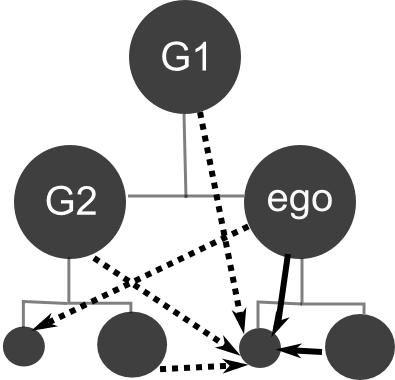
\includegraphics[width=0.5\textwidth]{Fig1.png}
\caption{Circles represent actors in the simulation and bars represent the kinship links between them.  The larger circles in the third generation represent care-giving offspring.  Solid lines show residence independent caring relationships, while dotted lines show caring relationships unique to the natal household.  Note, the number of offspring starts at 0 and grows throughout the simulation.}
\label{fig:kin_diag}       % Give a unique label
\end{figure}

The focus of this simulation is identifying how the source of care changes over time.  In particular, the model discriminates between care that is distributed among ego and her offspring, and care distributed outside that focal unit.  This discrimination is essential because care that stays within the focal unit is assumed to be residence independent, while the sources of care outside the focal unit are only available in the natal household.  During each distribution phase, the simulation records the amount of care that is distributed within the unit and the amount distributed outside the unit.  It should be noted that not only is care from G1 and G2 to ego's offspring viewed as a unique benefit to residing in the household, but also the care ego directs towards G2's offspring since that represents inclusive fitness benefits that could not be accrued living outside the household (see Figure \ref{fig:kin_diag}).

\section{Results}
\label{sec:2}

\begin{figure}[!ht]
  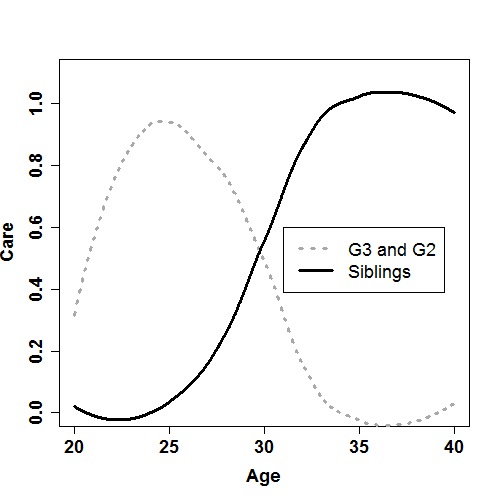
\includegraphics[width=0.75\textwidth]{Fig2.png}
\caption{Plot compares the mean amount of care coming from siblings to care coming from the G3 grandmother and G2 aunt and her offspring across the 20 year generation.}
\label{fig:simmns}
\end{figure}

\begin{figure}[!ht]
  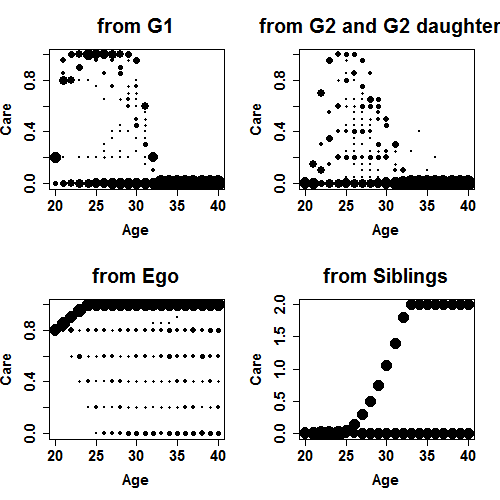
\includegraphics[width=0.75\textwidth]{Fig3.png}

\caption{Plots show the care given by different relative classes at each age across 100 simulated generations.  The level of clustering across simulations is indicated by the size of the points.}
\label{fig:simputs}
\end{figure}

The simulation finds that ego's care-based incentives unique to the natal household decrease with age (see Figure \ref{fig:simmns}).  The amount of outside care initially rises along with the likelihood of being burdened with a second dependent offspring, then decreases as earlier-born offspring reach an age where they can begin accepting some of the childcare responsibilities.  This shift happens because these older children's care crowds-out care coming from sources outside the focal unit.  Additionally, since both ego and her G2 sister are simultaneously experiencing a similar demographic shift, the opportunities to benefit through providing care to non-offspring also decreases from ego's perspective.   

While there is a clear downward trend with age across the simulations, there is considerable variation within a given simulation (see Figure \ref{fig:simputs}).  Due to the stochastic composition of kin groups resulting from the random reproductive rate of ego and G2, individuals may find themselves with limited care-based incentive in one year then significant incentive in the next. 
 
Increasing the rate of reproduction or including additional sisters both slightly decrease the initial incentive to remain home, but retains the same qualitative pattern seen above.  Placing the transition from needy to care-giving at an older age retains the eventual decrease, but delays it until later in the generation.  Adding the possibility of producing non-caring offspring (boys) has no significant effect on the pattern.  The assumption of linear increase in care with age may be inconsistent with the human case.  Research in both humans and non-human primates shows that mothers' ability to care improves dramatically after their first child \cite[p.~63]{hrdy2009mothers}.  If we adjust the simulation to fit this pattern the amount of outside care received in the early twenties increases to flatten out the initial bump in the curve without impacting the later age decline (see supplementary materials).

\section{Discussion}
\label{sec:3}

The results of this simulation show how in a cooperative care system where both secondary kin and siblings direct childcare assistance towards children, there are decreasing incentives to the natal camp as early-born children become reliable sources of care.  This demonstrates how childcare assistance may offer a powerful incentive towards philopatry early in a woman's reproductive career that tapers off over time.  Assuming some constant pressure to move away from home such as resource competition or the conflicting interests of husbands, the diminishing lure of childcare assistance helps explain the common forager residence pattern of initially living with the wife's family (``uxorilocality'') followed by a shift to the husband's family or a new household (``virilocality'' or ``neolocality'').  

Wood and Marlowe recently proposed an alternative model to explain this pattern that focuses on how women can expect more paternal investment while living in their husband's camp later in their reproductive careers than when they only have one or two children \cite{wood2011dynamics}.  Both the Wood and Marlowe model and the model proposed in this paper predict that women should be more open to virilocal residence when they have more children.  The factors in these models do not conflict in any way, and may both help explain the pattern of early uxorilocality and late virilocality.  However, the model put forward in this paper also helps explain cases where couples shift to a neolocal residence later in life, as well as cases where even unmarried women move away from home as they age. 

It is important to note that while I discuss this pattern of uxorilocal to virilocal residence, the modal pattern among foragers is more general flexibility with many residence shifts throughout life. Additionally, even among groups characterized by an “uxorilocal to virilocal” transition, this description disguises the tremendous flexibility of actual residence decisions.  Individuals among the Hadza, !Kung, and many other forager groups regularly shift residence throughout their lives.  Uxorilocal to virilocal merely captures the population-level trend in observed residence across the lifetime of individuals.  This perspective of a general trend with underlying residence stochasticity is consistent with another finding in our simulation.  Despite the expected decrease in household incentive with age, the incentive for ego to live at home varied widely within individual simulations at a given point in time.  This was a function of random variance in the rates of reproduction in the simulation, but the availability of childcare assistance in real life is likely to be much more variable.  The death of important sources of care, infant mortality, variable fertility, residence decisions of female relatives, and other factors would put individual women in situations where the incentives of childcare assistance in their familial camp are not consistent with simple age-based expectations.  This variable nature of childcare assistance as an incentive to philopatry allows for a system of facultative residence shifting at a much higher rate than implied by the mean decrease in expected childcare assistance with age.   

The variable and transient nature of childcare assistance as an incentive towards female philopatry has implications for the development of bilateral relationships between in-laws \cite{rodseth1991human}.  Chapais argues a central role for both sexes forming affinal relationships in the story of human evolution \cite{chapais2009primeval}.  Even in species characterized by sex-determinant dispersal patterns, individuals deviate from expectations when it is advantageous \cite{pusey1997influence}.  Stable residence incentives are conducive to social systems with simple dispersal rules.  In contrast, when the incentives to dispersal and philopatry are expected to change over time as I show with childcare assistance, more complex patterns may arise.  While females are expected to have a strong incentive to remain home early in life, males may see an advantage to retaining contact with their natal household even after dispersing to find a mate.  Not only is it likely that he can bring his mate to live with his kin later in life, but the dynamics of childcare in her household may allow at least a temporary visit to his familial household much sooner.  Initially dispersing males returning home with bonded females results in both members of a pair-bond being integrated into the household of their affines, allowing for bilateral affinity.  Chapais argues that the transition from female dispersal to bilateral affinity was the result of reciprocal exogamy and strong brother-sister bonds.  However, if a tendency towards early female philopatry resulted from the rising importance of childcare assistance, the nature of this particular incentive may offer an alternative explanation for the advent of bilateral affinity and whatever other traits cascade from that social adaptation.


%\begin{acknowledgements}
%If you'd like to thank anyone, place your comments here
%and remove the percent signs.
%\end{acknowledgements}

% BibTeX users please use one of
%\bibliographystyle{spmpsci}      % mathematics and physical sciences
%\bibliographystyle{spphys}       % APS-like style for physics
\bibliography{vashro_chilcaredynamics_refs}
\bibliographystyle{spbasic}      % basic style, author-year citations

\end{document}
% end of file template.tex

